\section{The RTEC language}\label{sec:RTEC-language}

The time model in RTEC is linear and includes integer time-points. Where \textttsmall{F} is a \emph{fluent}---a property that is allowed to have different values at different points in time---the term \textttsmall{F=V} denotes that fluent \textttsmall{F} has value \textttsmall{V}. Boolean fluents are a special case in which the possible values are \true\ and \false. \textttsmall{holdsAt(F=V, T)} represents that fluent \textttsmall{F} has value \textttsmall{V} at a particular time-point \textttsmall{T}. \textttsmall{holdsFor(F=V, I)} represents that \textttsmall{I} is the list of the maximal intervals for which \textttsmall{F=V} holds continuously. \holdsAt\ and \holdsFor\ are defined in such a way that, for any fluent \textttsmall{F}, \textttsmall{holdsAt(F=V, T)} if and only if \textttsmall{T} belongs to one of the maximal intervals of \textttsmall{I} for which \textttsmall{holdsFor(F=V, I)}. 

An \emph{event description} in RTEC includes rules that define the event instances with the use of the \happensAt\ predicate, the effects of events with the use of the \initiatedAt\ and \terminatedAt\ predicates, and the values of the fluents with the use of the \holdsAt\ and \holdsFor\ predicates, as well as other, possibly atemporal, constraints. Table~\ref{tbl:ec} summarises the RTEC predicates available to the event description developer. 

Fluents are either simple or statically determined. In brief, simple fluents are defined by means of \initiatedAt\ and \terminatedAt\ rules, while statically determined fluents are defined by means of application-dependent \holdsFor\ rules. More details on this distinction will be given shortly.

An event description is a (locally) stratified logic program \cite{local-strat}.
We restrict attention to \emph{hierarchical} event descriptions, those where it is possible to define a function \emph{level} that maps all fluent-values \textttsmall{F=V} and all events to the non-negative integers as follows. 
Events and statically determined fluent-values \textttsmall{F=V} of level $0$ are those whose  definitions do not depend on any other events or fluents. These represent the \emph{input entities}. There are no fluent-values \textttsmall{F=V} of simple fluents \textttsmall{F} in level $0$. 
Events and simple fluent-values of level $n$ ($n>0$) are defined in terms of at least one event or fluent-value of level $n{-}1$ and a possibly empty set of events and fluent-values from levels lower than $n{-}1$. Statically determined fluent-values of level $n$ are defined in terms of at least one fluent-value of level $n{-}1$ and a possibly empty set of fluent-values from levels lower than $n{-}1$. 
Events and fluent-values of level $n$ are the \emph{output entities}.
%Note that fluent-values $F\val V_i$ and $F\val V_j$ for $V_i{\neq}V_j$ could be mapped to different levels. For simplicity however, and without loss of generality, a fluent $F$ itself is either simple or statically determined but not both. 

In the following sections we present in more detail the building blocks of RTEC.

\begin{table}[t]
\caption{Main predicates of RTEC.}\vspace{-.3cm}\label{tbl:ec}
\begin{center}
\renewcommand{\arraystretch}{0.9}
\setlength\tabcolsep{3.8pt}
\begin{tabular}{ll}
\hline\noalign{\smallskip}
\multicolumn{1}{c}{\textbf{Predicate}} & \multicolumn{1}{c}{\textbf{Meaning}}  \\
\noalign{\smallskip}
\hline
\noalign{\smallskip}
\textttsmall{happensAt(E, T)} & Event \textttsmall{E} occurs at time \textttsmall{T}  \\[4pt]

%\textsf{\footnotesize initially}$(F \val V)$ & The value of fluent $F$ is $V$ at time $0$  \\[4pt]

\textttsmall{holdsAt(F=V, T)} & The value of fluent \textttsmall{F} is \textttsmall{V} at time \textttsmall{T} \\[4pt]

\textttsmall{holdsFor(F=V, I)} & \textttsmall{I} is the list of the maximal intervals \\
                           & for which \textttsmall{F=V} holds continuously\\[4pt]

\textttsmall{initiatedAt(F=V, T)} & At time \textttsmall{T} a period of time for which\\
& \textttsmall{F=V} is initiated \\[4pt]

\textttsmall{terminatedAt(F=V, T)} & At time \textttsmall{T} a period of time for which \\
& \textttsmall{F=V} is terminated \\[4pt]

\textttsmall{union\_all(L, I)} & \textttsmall{I} is the list of maximal intervals  \\
			    & produced by the union of the lists of \\
& maximal intervals of list \textttsmall{L} \\[4pt]

\textttsmall{intersect\_all(L, I)} & \textttsmall{I} is the list of maximal intervals \\
				& produced by the intersection of \\
& the lists of maximal intervals of list \textttsmall{L} \\[4pt]

\textttsmall{relative\_complement\_all(I', L, I)}	& \textttsmall{I} is the list of maximal intervals produced \\
	    & by the relative complement of the list   \\
				& of maximal intervals \textttsmall{I'} with respect to \\
 & every list of maximal intervals of list \textttsmall{L} \\[4pt]


%\abscomplementall$\mathit{(L,\ I)}$ & $I$ is the list of maximal intervals produced by\\
%				      & the absolute complement of each list of maximal intervals of list $L$ \\[5pt]
\hline
\end{tabular}
\end{center}
\end{table}

\subsection{Event Description}


\subsubsection{Events}

Events in RTEC are instantaneous and represented with the use of the \happensAt\ predicate. Our simple example has three events: \textttsmall{go\_to}, \textttsmall{lose\_wallet} and \textttsmall{win\_lottery}. 
Input events are indicated as \happensAt\ facts, i.e.~they have an empty body. In contrast, output events are defined by \happensAt\ rules, i.e.~rules with at least one body literal. %For instance, let's define the event ``explosion'' in terms of the two low-level fluents ``noise'' and ``temperature'':

%\begin{verbatim}
%happensAt(explosion(Room), T) :-
%    holdsAt(noise(Room)=high, T),
%    holdsAt(temperature(Room)=high, T).
%\end{verbatim}

\subsubsection{Fluents}

As already mentioned, fluents are either simple or statically determined.

\textbf{Simple Fluents.} 
For a simple fluent \textttsmall{F}, \textttsmall{F=V} holds at a particular time-point \textttsmall{T} if \textttsmall{F=V} has been \emph{initiated} by an event that has occurred at some time-point earlier than \textttsmall{T}, and has not been \emph{terminated} at some other time-point in the meantime. This is an implementation of the law of inertia. 
To compute the \emph{intervals} \textttsmall{I} for which \textttsmall{F=V}, i.e.~\textttsmall{holdsFor(F=V, I)}, we find all time-points \textttsmall{Ts} at which \textttsmall{F=V} is initiated, and then, for each \textttsmall{Ts}, we compute the first time-point \textttsmall{Tf} after \textttsmall{Ts} at which \textttsmall{F=V} is terminated.
The time-points at which \textttsmall{F=V} is initiated (respectively terminated) are computed by means of domain-specific \initiatedAt\ (resp.~\terminatedAt) rules. 

In our example, \textttsmall{rich} is a simple fluent. 
The maximal intervals during which \textttsmall{rich(Person)=true} holds continuously are computed using the domain-independent implementation of \holdsFor\ from the \initiatedAt\ and \terminatedAt\ rules defining this fluent.

In addition to constraints on events, the bodies of \initiatedAt\ and \terminatedAt\ rules may specify constraints on fluents by means of the \holdsAt, \initiatedAt\ and \terminatedAt\ predicates.

\textbf{Statically Determined Fluents.}
Apart from the domain-independent definition of \holdsFor, an event description may include domain-specific \holdsFor\ rules, used to define the values of a fluent \textttsmall{F} in terms of the values of other fluents. We call such a fluent \textttsmall{F} \emph{statically determined}. 
\holdsFor\ rules of this kind make use of interval manipulation constructs. 
RTEC provides three such constructs: \unionall, \intersectall\ and \complementall (see the last three items of Table \ref{tbl:ec}). \textttsmall{union\_all(+L, -I)} computes the list \textttsmall{I} of maximal intervals representing the union of maximal intervals of the lists of list \textttsmall{L}. For instance: 

{\small
\begin{verbatim}
union_all([[(5,20), (26,30)],[(28,35)]], [(5,20), (26,35)])
\end{verbatim}
}

Recall that a term of the form \textttsmall{(Ts, Te)} in RTEC represents the closed-open interval $\mathit{[Ts, Te)}$. \textttsmall{I} in \textttsmall{union\_all(L, I)} is a list of maximal intervals that includes each time-point that is part of at least one list of \textttsmall{L}. See Figure \ref{fig:interval-manipulation}(a) for a visual illustration.

\textttsmall{intersect\_all(+L, -I)} computes the list \textttsmall{I} of maximal intervals such that \textttsmall{I} represents the intersection of maximal intervals of the lists of list \textttsmall{L}, as, e.g.:

{\small
\begin{verbatim}
intersect_all([[(26,31)], [(21,26),(30,40)]], [(30,31)])
\end{verbatim}
}

\textttsmall{I} in \textttsmall{intersect\_all(L, I)} is a list of maximal intervals that includes each time-point that is part of all lists of \textttsmall{L} (see Figure \ref{fig:interval-manipulation}(b)).

\textttsmall{relative\_complement\_all(+I', +L, -I)} computes the list \textttsmall{I} of maximal intervals such that \textttsmall{I} represents the relative complements of the list of maximal intervals \textttsmall{I'} with respect to the maximal intervals of the lists of list \textttsmall{L}. Below is an example of \complementall:

{\small
\begin{verbatim}
relative_complement_all([(5,20), (26,50)], [[(1,4),(18,22)],[(28,35)]], 
                        [(5,18),(26,28),(35,50)])
\end{verbatim}
}

\textttsmall{I} in \textttsmall{relative\_complement\_all(I', L, I)} is a list of maximal intervals that includes each time-point of \textttsmall{I'} that is not part of any list of \textttsmall{L} (see Figure \ref{fig:interval-manipulation}(c)).  

%\begin{figure}[t]
%    \centering
%    \includegraphics[width=.8\textwidth]{figures/RTEC-interval-manipulation}
%    \caption{A visual illustration of the three interval manipulation constructs of RTEC. In this example, there are two input fluent streams, $I_1$ and $I_2$. The output of the three interval manipulation constructs is shown above the dashed line.}
%    \label{fig:interval-manipulation}
%\end{figure}

\begin{figure}[tp]
\centering
\subfigure[Union.]{ 
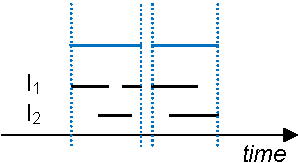
\includegraphics[width=0.31\textwidth]{figures/union}
%\label{fig:cer_replic_times}
}
\subfigure[Intersection.]{
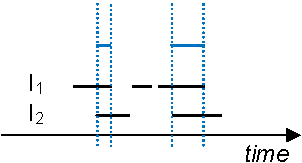
\includegraphics[width=0.31\textwidth]{figures/intersection}
%\label{fig:cer_replic_mem}
}
\subfigure[Relative Complement.]{
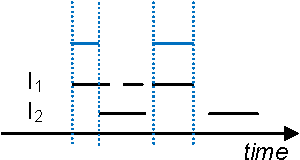
\includegraphics[width=0.31\textwidth]{figures/rcomplement}
%\label{fig:cer_replic_mes}
}
\caption{A visual illustration of the three interval manipulation constructs of RTEC. In this example, there are two input fluent streams, $I_1$ and $I_2$. The output of each interval manipulation construct is colored light blue.}
\label{fig:interval-manipulation}
\end{figure}


In our example, \textttsmall{happy} is a statically determined fluent defined by means of \unionall. 
However, this is just one way of defining happiness. For example, we could have specified that a person is happy when he is rich \textit{and} at the pub. To specify \textttsmall{happy} in this way one should replace \unionall\ by \intersectall\ in the \holdsFor\ rule of \textttsmall{happy}.

The interval manipulation constructs of RTEC support the following type of definition: for all time-points \textttsmall{T}, \textttsmall{F=V} holds at \textttsmall{T} if and only if some Boolean combination of fluent-value pairs holds at \textttsmall{T}. For a wide range of fluents, this is a much more concise definition than the traditional style of Event Calculus representation, i.e.~identifying the various conditions under which the fluent is initiated and terminated so that maximal intervals can then be computed using the domain-independent \holdsFor. Compare, e.g.~the statically determined fluent representation of \textttsmall{happy} in Listing~\ref{lst:rules} and the simple fluent representation below:

{\small
\begin{verbatim}
initiatedAt(happy(X)=true, T) :- 
    initiatedAt(rich(X)=true, T).
initiatedAt(happy(X)=true, T) :-
    initiatedAt(loc(X)=pub, T).
terminatedAt(happy(X)=true, T) :-
    terminatedAt(rich(X)=true, T)
    not holdsAt(loc(X)=pub, T).
terminatedAt(happy(X)=true, T) :-
    terminatedAt(loc(X)=pub, T),
    not holdsAt(rich(X)=true, T).
\end{verbatim}
}

\textttsmall{not} is negation by failure. The interval manipulation constructs of RTEC can also lead to much more efficient computation \cite{DBLP:journals/tkde/ArtikisSP15}.

\subsection{Declarations}\label{sec:declarations}

The declarations of our example were presented in Listing \ref{lst:declarations}.
In the declarations of an event description, we first need to denote the events, simple fluents and statically determined fluents. This is done with the use of the \textttsmall{event},  \textttsmall{simpleFluent} and \textttsmall{sDFluent} predicates.

%\subsubsection{Input Entities, Output Entities \& Indexing}

Each event and fluent must be declared as either \textttsmall{inputEntity} or \textttsmall{outputEntity}. As explained earlier in the section, the input entities may consist of events and/or statically determined fluents, while the output entities may comprise events, simple and/or statically determined fluents.

For each event and fluent, the user must also declare its \textttsmall{index}. In our example, \textttsmall{Person} is the index of all events and fluents. The index allows for the fast retrieval from the memory of the list of time-points, in the case of events, and maximal intervals, in the case of fluents. 

%\subsubsection{Grounding}

To perform query computation, RTEC grounds every output entity. This process is guided by the \textttsmall{grounding} predicate of the declarations language of RTEC, that denotes the domain of the variables of the output entities.  

%\subsubsection{Caching Order}

The final step in the declarations is to specify the \textttsmall{cachingOrder}, i.e.~the order in which the output entities will be processed. To take advantage of RTEC's caching technique, the output entities should be processed in a bottom-up manner. This way, when processing an output entity \textttsmall{U} of level $n$, the time-points/intervals of all entities defining \textttsmall{U}---these will all be in levels below $n$--- will simply be retrieved from the cache. 

Back to our example, if we look the rules, we will see that \textttsmall{happy} is defined in terms of \textttsmall{location} and \textttsmall{rich}. Thus, \textttsmall{location} and \textttsmall{rich} must must be processed before \textttsmall{happy}. \textttsmall{location} and \textttsmall{rich} are on the same level of the hierarchy and thus the order in which they are processed does not matter.
